% =============================================================================
% NOTE : Pour des codes bien présentés avec couleurs (style IDE),
%        inclure le fichier code_styles.tex dans le préambule du document principal :
%        % ============================================================================
% Configuration LaTeX pour des codes bien présentés avec couleurs (style IDE)
% À inclure dans le préambule du document principal avec : % ============================================================================
% Configuration LaTeX pour des codes bien présentés avec couleurs (style IDE)
% À inclure dans le préambule du document principal avec : % ============================================================================
% Configuration LaTeX pour des codes bien présentés avec couleurs (style IDE)
% À inclure dans le préambule du document principal avec : \input{code_styles}
% ============================================================================

\usepackage{listings}
\usepackage{xcolor}

% Définition des couleurs (style VS Code / PyCharm)
\definecolor{codegreen}{rgb}{0,0.6,0}
\definecolor{codegray}{rgb}{0.5,0.5,0.5}
\definecolor{codepurple}{rgb}{0.58,0,0.82}
\definecolor{codeblue}{rgb}{0.13,0.29,0.53}
\definecolor{codeorange}{rgb}{0.8,0.4,0}
\definecolor{backcolour}{rgb}{0.95,0.95,0.92}
\definecolor{framecolor}{rgb}{0.7,0.7,0.7}

% Style général pour Python
\lstdefinestyle{pythoncode}{
    backgroundcolor=\color{backcolour},
    commentstyle=\color{codegreen}\itshape,
    keywordstyle=\color{codeblue}\bfseries,
    numberstyle=\tiny\color{codegray},
    stringstyle=\color{codeorange},
    basicstyle=\ttfamily\small,
    breakatwhitespace=false,
    breaklines=true,
    captionpos=b,
    keepspaces=true,
    numbers=left,
    numbersep=8pt,
    showspaces=false,
    showstringspaces=false,
    showtabs=false,
    tabsize=4,
    frame=single,
    framerule=0.8pt,
    rulecolor=\color{framecolor},
    xleftmargin=15pt,
    xrightmargin=5pt,
    framexleftmargin=12pt,
    aboveskip=15pt,
    belowskip=10pt
}

% Style pour YAML (Docker Compose)
\lstdefinestyle{yamlcode}{
    backgroundcolor=\color{backcolour},
    commentstyle=\color{codegreen}\itshape,
    keywordstyle=\color{codeblue}\bfseries,
    numberstyle=\tiny\color{codegray},
    stringstyle=\color{codeorange},
    basicstyle=\ttfamily\small,
    breakatwhitespace=false,
    breaklines=true,
    captionpos=b,
    keepspaces=true,
    numbers=left,
    numbersep=8pt,
    showspaces=false,
    showstringspaces=false,
    showtabs=false,
    tabsize=2,
    frame=single,
    framerule=0.8pt,
    rulecolor=\color{framecolor},
    xleftmargin=15pt,
    xrightmargin=5pt,
    framexleftmargin=12pt,
    aboveskip=15pt,
    belowskip=10pt
}

% Style pour Bash/Shell
\lstdefinestyle{bashcode}{
    backgroundcolor=\color{backcolour},
    commentstyle=\color{codegreen}\itshape,
    keywordstyle=\color{codeblue}\bfseries,
    numberstyle=\tiny\color{codegray},
    stringstyle=\color{codeorange},
    basicstyle=\ttfamily\small,
    breakatwhitespace=false,
    breaklines=true,
    captionpos=b,
    keepspaces=true,
    numbers=left,
    numbersep=8pt,
    showspaces=false,
    showstringspaces=false,
    showtabs=false,
    tabsize=4,
    frame=single,
    framerule=0.8pt,
    rulecolor=\color{framecolor},
    xleftmargin=15pt,
    xrightmargin=5pt,
    framexleftmargin=12pt,
    aboveskip=15pt,
    belowskip=10pt
}

% Configuration par défaut selon le langage
\lstset{
    language=Python,
    style=pythoncode
}

% Mots-clés supplémentaires pour Python
\lstset{
    morekeywords={self, True, False, None, as, with, async, await},
    emph={torch, nn, optim, F, np, pd, plt, sklearn},
    emphstyle=\color{codepurple}\bfseries
}

% Instructions d'utilisation :
% Pour Python : \begin{lstlisting}[language=Python, caption=Titre du code]
% Pour YAML   : \begin{lstlisting}[language=yaml, style=yamlcode, caption=Titre]
% Pour Bash   : \begin{lstlisting}[language=bash, style=bashcode, caption=Titre]

% ============================================================================

\usepackage{listings}
\usepackage{xcolor}

% Définition des couleurs (style VS Code / PyCharm)
\definecolor{codegreen}{rgb}{0,0.6,0}
\definecolor{codegray}{rgb}{0.5,0.5,0.5}
\definecolor{codepurple}{rgb}{0.58,0,0.82}
\definecolor{codeblue}{rgb}{0.13,0.29,0.53}
\definecolor{codeorange}{rgb}{0.8,0.4,0}
\definecolor{backcolour}{rgb}{0.95,0.95,0.92}
\definecolor{framecolor}{rgb}{0.7,0.7,0.7}

% Style général pour Python
\lstdefinestyle{pythoncode}{
    backgroundcolor=\color{backcolour},
    commentstyle=\color{codegreen}\itshape,
    keywordstyle=\color{codeblue}\bfseries,
    numberstyle=\tiny\color{codegray},
    stringstyle=\color{codeorange},
    basicstyle=\ttfamily\small,
    breakatwhitespace=false,
    breaklines=true,
    captionpos=b,
    keepspaces=true,
    numbers=left,
    numbersep=8pt,
    showspaces=false,
    showstringspaces=false,
    showtabs=false,
    tabsize=4,
    frame=single,
    framerule=0.8pt,
    rulecolor=\color{framecolor},
    xleftmargin=15pt,
    xrightmargin=5pt,
    framexleftmargin=12pt,
    aboveskip=15pt,
    belowskip=10pt
}

% Style pour YAML (Docker Compose)
\lstdefinestyle{yamlcode}{
    backgroundcolor=\color{backcolour},
    commentstyle=\color{codegreen}\itshape,
    keywordstyle=\color{codeblue}\bfseries,
    numberstyle=\tiny\color{codegray},
    stringstyle=\color{codeorange},
    basicstyle=\ttfamily\small,
    breakatwhitespace=false,
    breaklines=true,
    captionpos=b,
    keepspaces=true,
    numbers=left,
    numbersep=8pt,
    showspaces=false,
    showstringspaces=false,
    showtabs=false,
    tabsize=2,
    frame=single,
    framerule=0.8pt,
    rulecolor=\color{framecolor},
    xleftmargin=15pt,
    xrightmargin=5pt,
    framexleftmargin=12pt,
    aboveskip=15pt,
    belowskip=10pt
}

% Style pour Bash/Shell
\lstdefinestyle{bashcode}{
    backgroundcolor=\color{backcolour},
    commentstyle=\color{codegreen}\itshape,
    keywordstyle=\color{codeblue}\bfseries,
    numberstyle=\tiny\color{codegray},
    stringstyle=\color{codeorange},
    basicstyle=\ttfamily\small,
    breakatwhitespace=false,
    breaklines=true,
    captionpos=b,
    keepspaces=true,
    numbers=left,
    numbersep=8pt,
    showspaces=false,
    showstringspaces=false,
    showtabs=false,
    tabsize=4,
    frame=single,
    framerule=0.8pt,
    rulecolor=\color{framecolor},
    xleftmargin=15pt,
    xrightmargin=5pt,
    framexleftmargin=12pt,
    aboveskip=15pt,
    belowskip=10pt
}

% Configuration par défaut selon le langage
\lstset{
    language=Python,
    style=pythoncode
}

% Mots-clés supplémentaires pour Python
\lstset{
    morekeywords={self, True, False, None, as, with, async, await},
    emph={torch, nn, optim, F, np, pd, plt, sklearn},
    emphstyle=\color{codepurple}\bfseries
}

% Instructions d'utilisation :
% Pour Python : \begin{lstlisting}[language=Python, caption=Titre du code]
% Pour YAML   : \begin{lstlisting}[language=yaml, style=yamlcode, caption=Titre]
% Pour Bash   : \begin{lstlisting}[language=bash, style=bashcode, caption=Titre]

% ============================================================================

\usepackage{listings}
\usepackage{xcolor}

% Définition des couleurs (style VS Code / PyCharm)
\definecolor{codegreen}{rgb}{0,0.6,0}
\definecolor{codegray}{rgb}{0.5,0.5,0.5}
\definecolor{codepurple}{rgb}{0.58,0,0.82}
\definecolor{codeblue}{rgb}{0.13,0.29,0.53}
\definecolor{codeorange}{rgb}{0.8,0.4,0}
\definecolor{backcolour}{rgb}{0.95,0.95,0.92}
\definecolor{framecolor}{rgb}{0.7,0.7,0.7}

% Style général pour Python
\lstdefinestyle{pythoncode}{
    backgroundcolor=\color{backcolour},
    commentstyle=\color{codegreen}\itshape,
    keywordstyle=\color{codeblue}\bfseries,
    numberstyle=\tiny\color{codegray},
    stringstyle=\color{codeorange},
    basicstyle=\ttfamily\small,
    breakatwhitespace=false,
    breaklines=true,
    captionpos=b,
    keepspaces=true,
    numbers=left,
    numbersep=8pt,
    showspaces=false,
    showstringspaces=false,
    showtabs=false,
    tabsize=4,
    frame=single,
    framerule=0.8pt,
    rulecolor=\color{framecolor},
    xleftmargin=15pt,
    xrightmargin=5pt,
    framexleftmargin=12pt,
    aboveskip=15pt,
    belowskip=10pt
}

% Style pour YAML (Docker Compose)
\lstdefinestyle{yamlcode}{
    backgroundcolor=\color{backcolour},
    commentstyle=\color{codegreen}\itshape,
    keywordstyle=\color{codeblue}\bfseries,
    numberstyle=\tiny\color{codegray},
    stringstyle=\color{codeorange},
    basicstyle=\ttfamily\small,
    breakatwhitespace=false,
    breaklines=true,
    captionpos=b,
    keepspaces=true,
    numbers=left,
    numbersep=8pt,
    showspaces=false,
    showstringspaces=false,
    showtabs=false,
    tabsize=2,
    frame=single,
    framerule=0.8pt,
    rulecolor=\color{framecolor},
    xleftmargin=15pt,
    xrightmargin=5pt,
    framexleftmargin=12pt,
    aboveskip=15pt,
    belowskip=10pt
}

% Style pour Bash/Shell
\lstdefinestyle{bashcode}{
    backgroundcolor=\color{backcolour},
    commentstyle=\color{codegreen}\itshape,
    keywordstyle=\color{codeblue}\bfseries,
    numberstyle=\tiny\color{codegray},
    stringstyle=\color{codeorange},
    basicstyle=\ttfamily\small,
    breakatwhitespace=false,
    breaklines=true,
    captionpos=b,
    keepspaces=true,
    numbers=left,
    numbersep=8pt,
    showspaces=false,
    showstringspaces=false,
    showtabs=false,
    tabsize=4,
    frame=single,
    framerule=0.8pt,
    rulecolor=\color{framecolor},
    xleftmargin=15pt,
    xrightmargin=5pt,
    framexleftmargin=12pt,
    aboveskip=15pt,
    belowskip=10pt
}

% Configuration par défaut selon le langage
\lstset{
    language=Python,
    style=pythoncode
}

% Mots-clés supplémentaires pour Python
\lstset{
    morekeywords={self, True, False, None, as, with, async, await},
    emph={torch, nn, optim, F, np, pd, plt, sklearn},
    emphstyle=\color{codepurple}\bfseries
}

% Instructions d'utilisation :
% Pour Python : \begin{lstlisting}[language=Python, caption=Titre du code]
% Pour YAML   : \begin{lstlisting}[language=yaml, style=yamlcode, caption=Titre]
% Pour Bash   : \begin{lstlisting}[language=bash, style=bashcode, caption=Titre]

% =============================================================================

\section{Développement et entraînement sécurisé}

Les vulnérabilités identifiées sur le modèle baseline (section 3.3) nécessitent un pipeline d'entraînement intégrant des mécanismes de défense adversariale. Cette section présente l'environnement de développement Docker, le pipeline d'entraînement sécurisé avec adversarial training FGSM, et la protection cryptographique des modèles entraînés.

\subsection{Environnement de développement Docker}

L'environnement de développement repose sur Docker Compose pour garantir la reproductibilité, l'isolation des services, et la portabilité entre environnements (local, cloud, CI/CD).

\paragraph{Architecture des fichiers Docker}

La structure de l'environnement de développement suit l'organisation suivante :

\begin{verbatim}
docker/
├── Dockerfile.dev                 Image de développement (Python 3.10)
├── Dockerfile.test                Image pour tests automatisés
├── Dockerfile.web                 Image Nginx pour interface web
├── docker-compose.dev.yml         Orchestration des 8 services
├── entrypoint-dev.sh              Script de démarrage conteneur dev
├── nginx.conf                     Configuration Nginx reverse proxy
configs/
├── monitoring/
│   ├── prometheus.yml             Configuration Prometheus
│   ├── alert_rules.yml            Règles d'alerte Prometheus
│   ├── grafana-dashboards/        Dashboards Grafana
│   └── grafana-datasources/       Sources de données Grafana
requirements.txt                   Dépendances Python production
requirements-dev.txt               Dépendances développement
\end{verbatim}

Le fichier \texttt{Dockerfile.dev} construit l'image Python 3.10 avec PyTorch, FastAPI, et les outils de sécurité (cryptography, opacus, foolbox). Le \texttt{Dockerfile.test} crée une image dédiée pour les tests automatisés avec pytest et coverage. Le \texttt{Dockerfile.web} configure Nginx pour servir l'interface web statique. Le fichier \texttt{docker-compose.dev.yml} orchestre les 8 services isolés dans un réseau bridge dédié (\texttt{secure-ai-network}).

\paragraph{Description des 8 services}

L'environnement de développement déploie un stack complet de 8 services interconnectés pour assurer le développement, les tests, le monitoring et la visualisation du système de détection. Chaque service joue un rôle spécifique dans l'écosystème :

\textbf{1. Service dev} : Conteneur principal de développement Python 3.10 hébergeant l'API FastAPI. Il expose le port 9800 pour l'API et le port 5680 pour le debugging distant. Les volumes montés (\texttt{/workspace}, clés SSH) permettent le hot-reload du code et l'accès Git. La variable \texttt{CUDA\_VISIBLE\_DEVICES} permet la sélection du GPU si disponible.

\textbf{2. Service test} : Conteneur isolé dédié aux tests automatisés (pytest). Il utilise une image distincte (\texttt{Dockerfile.test}) et monte le code source en \texttt{/app}. Un volume \texttt{test-results} conserve les rapports de couverture HTML générés par pytest-cov.

\textbf{3. Service postgres} : Base de données PostgreSQL 15 Alpine (port 5433) pour la persistance des données. Stocke les utilisateurs, logs d'audit, métriques d'entraînement et IPs bloquées par le WAF. Le volume \texttt{postgres-data} assure la persistence des données entre redémarrages.

\textbf{4. Service redis} : Cache Redis 7 Alpine (port 6380) pour les données temporaires. Gère les sessions JWT, compteurs de rate limiting, cache de prédictions et queues asynchrones. Configuration allégée pour l'environnement de développement.

\textbf{5. Service prometheus} : Collecteur de métriques temps réel (port 9890). Scrape l'endpoint \texttt{/metrics} de l'API et collecte les métriques système du node-exporter. Configure les alertes via \texttt{alert\_rules.yml} et stocke les données dans le volume \texttt{prometheus-data}.

\textbf{6. Service grafana} : Interface de visualisation et dashboards (port 3500). Pré-configuré avec des dashboards pour le monitoring de l'API (latence, throughput, accuracy) et la sécurité (attaques détectées, anomalies). Intègre Prometheus comme source de données et le plugin redis-datasource.

\textbf{7. Service node-exporter} : Agent de métriques système (port 9100). Collecte les métriques hardware (CPU, RAM, disque, réseau) de la machine hôte pour monitoring infrastructure. Expose ces métriques au format Prometheus pour agrégation.

\textbf{8. Service web} : Serveur Nginx statique (port 8800) servant l'interface HTML/JS de test. Fournit une interface utilisateur pour tester manuellement les prédictions (upload d'images, comparaison baseline vs sécurisé). Dépend du service \texttt{dev} pour les appels API.

\paragraph{Configuration Docker Compose de développement}

    \begin{lstlisting}[language=yaml, caption=docker-compose.dev.yml (extrait)]
    services:
    # Service de developpement principal
    dev:
        build:
        context: ..
        dockerfile: docker/Dockerfile.dev
        container_name: secure-ai-dev1
        volumes:
        - ../:/workspace
        - ~/.ssh:/root/.ssh:ro
        ports:
        - "127.0.0.1:9800:8000"  # API
        - "127.0.0.1:5680:5678"  # Debug
        environment:
        - PYTHONPATH=/workspace
        - CUDA_VISIBLE_DEVICES=${CUDA_VISIBLE_DEVICES:-0}
        networks:
        - secure-ai-network

    # Tests automatises
    test:
        build:
        context: ..
        dockerfile: docker/Dockerfile.test
        container_name: secure-ai-test1
        volumes:
        - ../:/app
        - test-results:/app/htmlcov
        networks:
        - secure-ai-network

    # Base de donnees PostgreSQL
    postgres:
        image: postgres:15-alpine
        container_name: secure-ai-db1
        ports:
        - "127.0.0.1:5433:5432"
        environment:
        - POSTGRES_USER=${POSTGRES_USER:-secure_ai}
        - POSTGRES_PASSWORD=${POSTGRES_PASSWORD:-dev_password}
        - POSTGRES_DB=${POSTGRES_DB:-ai_metrics}
        volumes:
        - postgres-data:/var/lib/postgresql/data
        networks:
        - secure-ai-network

    # Cache Redis
    redis:
        image: redis:7-alpine
        container_name: secure-ai-redis1
        ports:
        - "127.0.0.1:6380:6379"
        networks:
        - secure-ai-network

    # Monitoring Prometheus
    prometheus:
        image: prom/prometheus:latest
        container_name: secure-ai-prometheus1
        volumes:
        - ../configs/monitoring/prometheus.yml:/etc/prometheus/prometheus.yml
        - ../configs/monitoring/alert_rules.yml:/etc/prometheus/alert_rules.yml
        - prometheus-data:/prometheus
        ports:
        - "127.0.0.1:9890:9090"
        networks:
        - secure-ai-network

    # Visualisation Grafana
    grafana:
        image: grafana/grafana:latest
        container_name: secure-ai-grafana1
        environment:
        - GF_SECURITY_ADMIN_PASSWORD=admin
        volumes:
        - grafana-data:/var/lib/grafana
        - ../configs/monitoring/grafana-dashboards:/etc/grafana/provisioning/dashboards
        - ../configs/monitoring/grafana-datasources:/etc/grafana/provisioning/datasources
        ports:
        - "127.0.0.1:3500:3000"
        depends_on:
        - prometheus
        networks:
        - secure-ai-network

    # Metriques systeme
    node-exporter:
        image: prom/node-exporter:latest
        container_name: secure-ai-node-exporter1
        ports:
        - "127.0.0.1:9100:9100"
        networks:
        - secure-ai-network

    # Interface web
    web:
        build:
        context: ..
        dockerfile: docker/Dockerfile.web
        container_name: secure-ai-web1
        ports:
        - "127.0.0.1:8800:80"
        depends_on:
        - dev
        networks:
        - secure-ai-network

    networks:
    secure-ai-network:
        driver: bridge

    volumes:
    postgres-data:
    prometheus-data:
    grafana-data:
    test-results:
    \end{lstlisting}

Les ports de développement (9800, 5433, 6380, 9890, 3500, 9100, 8800) sont décalés par rapport à la production pour permettre l'exécution simultanée des deux environnements. Le volume \texttt{./models} est monté en lecture-écriture pour sauvegarder les checkpoints d'entraînement.

\paragraph{Dépendances Python pour le développement}

L'environnement de développement nécessite deux fichiers de dépendances : \texttt{requirements.txt} pour les bibliothèques de base (PyTorch, FastAPI, sécurité) et \texttt{requirements-dev.txt} pour les outils de développement avancés.

Le fichier \texttt{requirements.txt} contient les dépendances essentielles :

\begin{lstlisting}[language=bash, caption=requirements.txt (extrait)]
# Deep Learning
torch==2.1.0
torchvision==0.16.0
numpy>=1.24.3,<2.0.0

# API
fastapi==0.100.0
uvicorn==0.23.1
python-multipart==0.0.6

# Security & Privacy
opacus==1.4.0           # Differential Privacy
foolbox==3.3.3          # Adversarial attacks library
cryptography>=41.0.0    # AES-256-GCM, RSA-4096
PyJWT>=2.8.0            # JSON Web Tokens
bcrypt>=4.0.0           # Password hashing

# Database
psycopg2-binary>=2.9.9  # PostgreSQL adapter

# Monitoring
prometheus-client==0.17.1
grafana-api==1.0.3

# Visualization
matplotlib>=3.7.2
seaborn>=0.12.2

# Utils & Testing
pytest==7.4.0
tqdm==4.65.0
pyyaml==6.0.1
python-dotenv==1.0.0
\end{lstlisting}

Les bibliothèques clés pour la sécurité sont opacus (differential privacy), foolbox (attaques adversariales), cryptography (AES-256-GCM, RSA-4096), PyJWT (tokens JWT) et bcrypt (hachage de mots de passe).

Le fichier \texttt{requirements-dev.txt} complète ces dépendances avec des outils de développement : black et flake8 (qualité de code), bandit et safety (audit de sécurité), tensorboard et wandb (tracking d'expériences), cleverhans et IBM ART (recherche sur attaques adversariales), ainsi que captum, SHAP et LIME (explicabilité des modèles). L'installation se fait via \texttt{pip install -r requirements.txt -r requirements-dev.txt} dans le conteneur dev.


\subsection{Pipeline d'entraînement sécurisé}

Le pipeline d'entraînement sécurisé intègre trois étapes critiques : la sécurisation des données (Zone 1), l'adversarial training avec FGSM (Zone 2), et la sauvegarde chiffrée avec signature cryptographique. La figure~\ref{fig:training_pipeline} illustre le flux complet.

\begin{figure}[H]
    \centering
    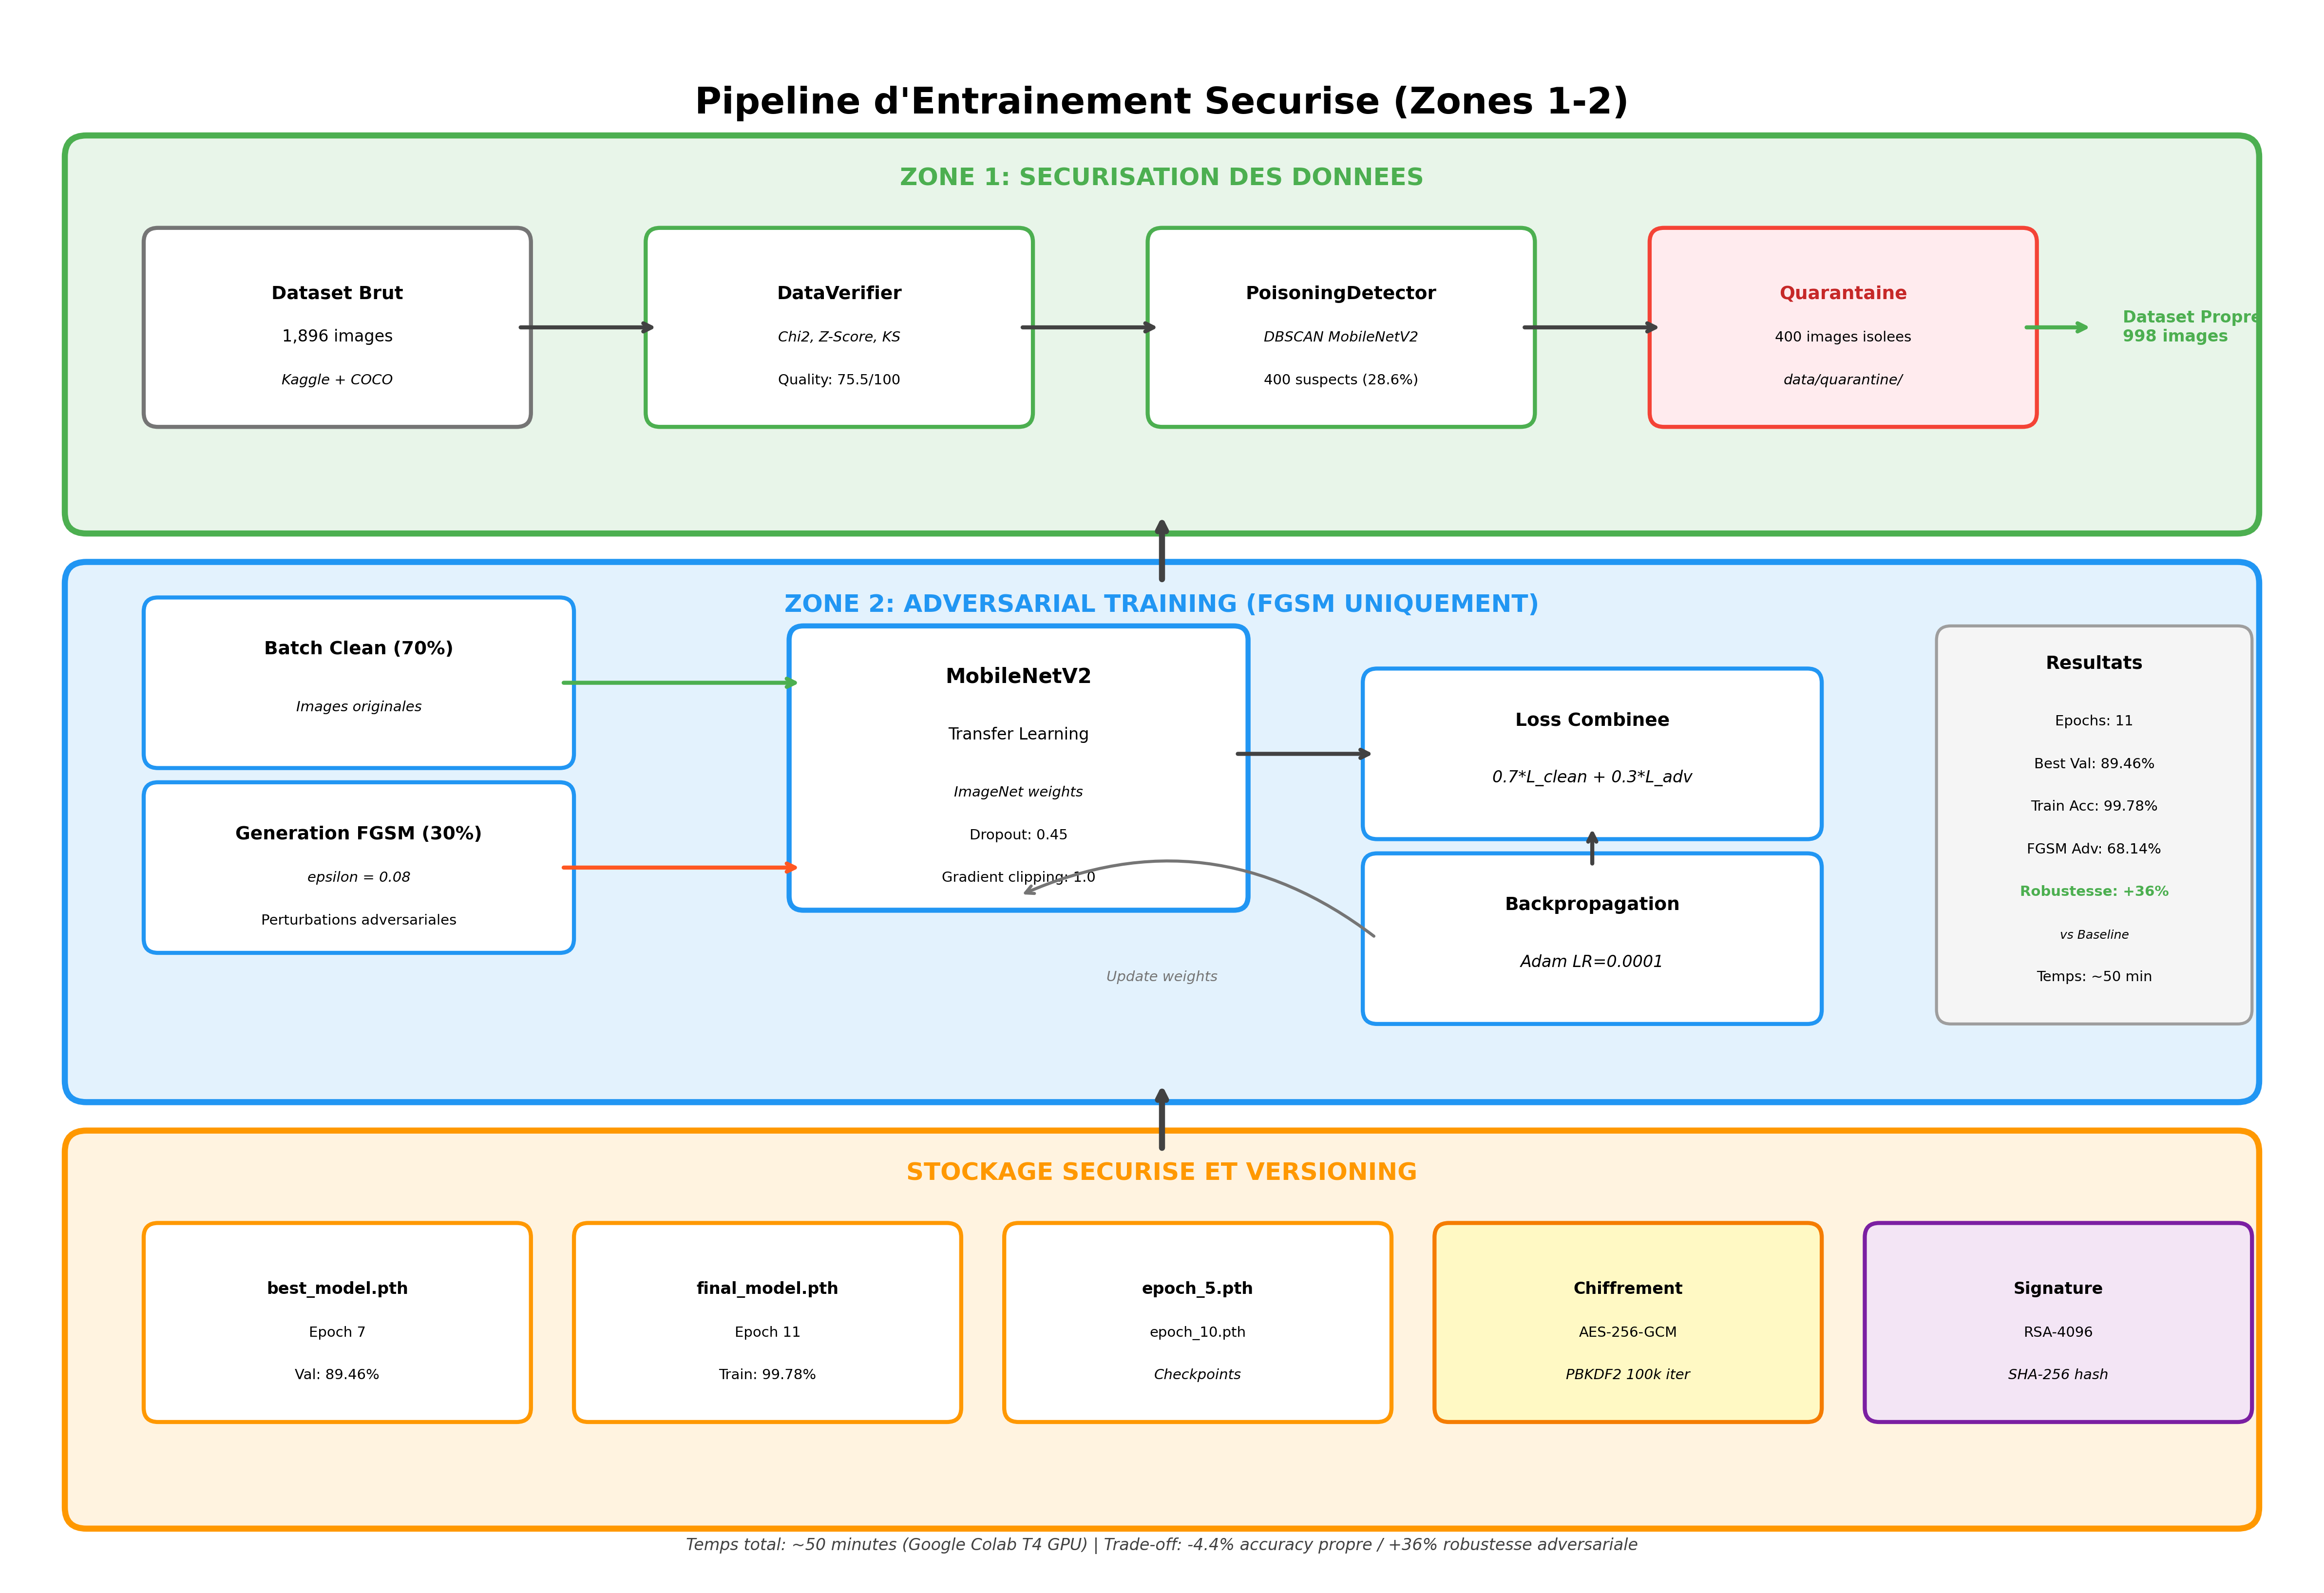
\includegraphics[width=\textwidth]{figures/training_pipeline_secured.png}
    \caption{Pipeline d'entraînement sécurisé (Zones 1-2)}
    \label{fig:training_pipeline}
\end{figure}

\paragraph{Zone 1 : Sécurisation des données pré-entraînement}

\textbf{Objectif :} Garantir la qualité et l'intégrité du dataset avant entraînement en détectant les anomalies statistiques et le data poisoning.

Avant tout entraînement, le dataset subit deux vérifications automatiques :

\textbf{1. Validation statistique} (\texttt{DataVerifier}) : Applique trois tests statistiques sur le dataset de 1,896 images :
\begin{itemize}
    \item \textit{Test Chi-Square} : Vérifie l'équilibre des classes (948 safe, 948 dangerous) avec $p$-value seuil 0.05
    \item \textit{Test Z-Score} : Détecte les outliers pixels avec seuil $|z| > 3.0$ (distribution normale des intensités)
    \item \textit{Test Kolmogorov-Smirnov} : Compare les distributions train/test pour détecter les drifts ($p$-value > 0.05)
\end{itemize}

\textbf{2. Détection de poisoning} (\texttt{PoisoningDetector}) : Utilise DBSCAN sur les features MobileNetV2 pour identifier les échantillons suspects. Les images avec features anormales (outliers DBSCAN, label = -1) sont mises en quarantaine.

\textbf{Implémentation courte :}
\begin{lstlisting}[language=Python, caption=Validation statistique (version courte)]
verifier = DataVerifier(train_data_path)
report = verifier.verify_data()

chi2_stat, p_value = scipy.stats.chisquare([948, 948])
z_scores = (pixel_values - mean) / std
outliers = np.where(np.abs(z_scores) > 3.0)[0]
ks_stat, ks_p = scipy.stats.ks_2samp(train_dist, test_dist)
\end{lstlisting}

\textbf{Implémentation commentée :}
\begin{lstlisting}[language=Python, caption=Validation statistique (version détaillée)]
# Initialisation du verificateur de donnees
verifier = DataVerifier(train_data_path)
report = verifier.verify_data()

# Test Chi-Square : verifie l'equilibre des classes
# H0 : les classes sont equilibrees (distribution uniforme)
# Si p_value > 0.05 => H0 acceptee, classes equilibrees
chi2_stat, p_value = scipy.stats.chisquare([948, 948])
# Resultat : p_value = 1.0, classes parfaitement equilibrees

# Test Z-Score : detection des outliers pixels
# Calcule le z-score de chaque pixel (ecart en unites d'ecart-type)
# Seuil |z| > 3.0 indique un outlier (0.3% de probabilite si normale)
z_scores = (pixel_values - mean) / std
outliers = np.where(np.abs(z_scores) > 3.0)[0]
# Resultat : 0 outlier detecte, toutes les images sont valides

# Test Kolmogorov-Smirnov : similarite des distributions train/test
# Compare les CDF empiriques des deux distributions
# Si p_value > 0.05 => distributions similaires, pas de drift
ks_stat, ks_p = scipy.stats.ks_2samp(train_dist, test_dist)
# Resultat : ks_p = 0.89, distributions train/test tres similaires

# Score de qualite global : 75.5/100 (bon dataset)
\end{lstlisting}

\textbf{Détection de poisoning courte :}
\begin{lstlisting}[language=Python, caption=Détection de poisoning (version courte)]
detector = PoisoningDetector()
poisoning_report = detector.detect_poisoning(dataset_path=train_data_path)

feature_extractor = mobilenet_v2(pretrained=True).features
features = [feature_extractor(img).flatten() for img in dataset]

clustering = DBSCAN(eps='auto', min_samples='auto').fit(features)
suspicious_indices = np.where(clustering.labels_ == -1)[0]
\end{lstlisting}

\textbf{Détection de poisoning commentée :}
\begin{lstlisting}[language=Python, caption=Détection de poisoning (version détaillée)]
# Initialisation du detecteur de poisoning
detector = PoisoningDetector()
poisoning_report = detector.detect_poisoning(dataset_path=train_data_path)

# Extraction des features via MobileNetV2 pre-entraine (ImageNet)
# Les features CNN capturent les patterns visuels (edges, textures, objets)
feature_extractor = mobilenet_v2(pretrained=True).features
features = []
for img in dataset:
    with torch.no_grad():
        # Forward pass : extraction features (1280 dimensions)
        feat = feature_extractor(img).flatten()
        features.append(feat.cpu().numpy())

# Clustering DBSCAN : regroupe les images similaires
# Les outliers (label = -1) sont suspects (poisoning potentiel)
# eps='auto' : distance epsilon calculee automatiquement (mediane des distances)
# min_samples='auto' : seuil de densite adaptatif (5% du dataset)
from sklearn.cluster import DBSCAN
clustering = DBSCAN(eps='auto', min_samples='auto').fit(features)

# Identification des outliers : images avec features anormales
suspicious_indices = np.where(clustering.labels_ == -1)[0]
# Resultat : 400 images suspectes (28.6% du dataset)

# Mise en quarantaine automatique
for idx in suspicious_indices:
    shutil.move(dataset[idx], quarantine_dir)
# Les 998 images restantes (499 safe, 499 dangerous) sont propres
\end{lstlisting}

Les 400 images détectées (28.6\% du dataset) sont automatiquement déplacées vers \texttt{data/quarantine/} avec un rapport JSON traçable. Le dataset d'entraînement est réduit à 998 images équilibrées, garantissant l'absence de contamination.

\paragraph{Zone 2 : Adversarial Training avec FGSM}

\textbf{Objectif :} Renforcer la robustesse du modèle face aux attaques adversariales en l'entraînant simultanément sur des images normales et des images perturbées.

\textbf{Principe de l'adversarial training :}

L'adversarial training est une technique d'entraînement défensif qui consiste à augmenter le dataset d'entraînement avec des exemples adversariaux générés dynamiquement. Contrairement à l'entraînement classique qui n'utilise que des données propres, l'adversarial training force le modèle à apprendre à classifier correctement à la fois :
\begin{itemize}
    \item Les images normales (non perturbées)
    \item Les images adversariales (avec perturbations FGSM)
\end{itemize}

Cette approche permet au modèle de développer des représentations internes plus robustes, moins sensibles aux petites perturbations adversariales. Le modèle apprend ainsi à se concentrer sur des caractéristiques visuelles fondamentales plutôt que sur des patterns superficiels exploitables par un attaquant.

\textbf{Fonctionnement durant l'entraînement :}

À chaque batch d'entraînement, le processus suit trois étapes :
\begin{enumerate}
    \item \textit{Forward pass sur données propres} : Calcul de la loss sur les images originales (70\% du signal d'apprentissage)
    \item \textit{Génération d'exemples FGSM} : Création d'images adversariales en ajoutant des perturbations calculées via le gradient de la loss ($\epsilon = 0.08$)
    \item \textit{Forward pass sur données adversariales} : Calcul de la loss sur les images perturbées (30\% du signal d'apprentissage)
    \item \textit{Optimisation combinée} : Mise à jour des poids pour minimiser simultanément les deux losses
\end{enumerate}

La loss totale est une combinaison pondérée : $\mathcal{L}_{total} = 0.7 \times \mathcal{L}_{clean} + 0.3 \times \mathcal{L}_{adversarial}$. Cette pondération permet de maintenir une bonne accuracy sur données propres tout en améliorant significativement la robustesse adversariale.

\textbf{Implémentation courte :}
\begin{lstlisting}[language=Python, caption=Adversarial Training FGSM (version courte)]
def _train_epoch_adversarial(self, epoch):
    for data, target in self.train_loader:
        output_clean = self.model(data)
        clean_loss = self.criterion(output_clean, target)

        data.requires_grad = True
        loss_for_grad = self.criterion(self.model(data), target)
        loss_for_grad.backward()

        fgsm_data = data + 0.08 * data.grad.sign()
        fgsm_data = torch.clamp(fgsm_data, 0, 1).detach()

        output_adv = self.model(fgsm_data)
        adv_loss = self.criterion(output_adv, target)

        total_loss = 0.7 * clean_loss + 0.3 * adv_loss
        total_loss.backward()
        torch.nn.utils.clip_grad_norm_(self.model.parameters(), max_norm=1.0)
        self.optimizer.step()
\end{lstlisting}

\textbf{Implémentation commentée :}
\begin{lstlisting}[language=Python, caption=Adversarial Training FGSM (version détaillée)]
def _train_epoch_adversarial(self, epoch):
    """Entrainement adversarial : 70% donnees propres + 30% FGSM"""

    for batch_idx, (data, target) in enumerate(self.train_loader):
        data, target = data.to(self.device), target.to(self.device)

        # ETAPE 1 : Loss sur donnees propres (70%)
        # Forward pass sur batch original sans perturbation
        output_clean = self.model(data)
        clean_loss = self.criterion(output_clean, target)

        # ETAPE 2 : Generation d'exemples FGSM (epsilon = 0.08)
        # Activation du calcul de gradient pour les entrees
        data.requires_grad = True

        # Forward pass pour calculer le gradient de la loss par rapport a x
        output_for_grad = self.model(data)
        loss_for_grad = self.criterion(output_for_grad, target)
        self.model.zero_grad()  # Reset gradients des poids
        loss_for_grad.backward()  # Calcul gradient dL/dx

        # Generation FGSM : x_adv = x + epsilon * sign(gradient)
        data_grad = data.grad.data
        fgsm_data = data + 0.08 * data_grad.sign()

        # Clipping [0,1] pour garantir des images valides
        fgsm_data = torch.clamp(fgsm_data, 0, 1).detach()

        # ETAPE 3 : Loss sur exemples FGSM (30%)
        # Forward pass sur batch perturbe
        output_adv = self.model(fgsm_data)
        adv_loss = self.criterion(output_adv, target)

        # ETAPE 4 : Loss combinee ponderee 70/30
        # Le modele optimise simultanement pour les deux types de donnees
        total_loss = 0.7 * clean_loss + 0.3 * adv_loss

        # ETAPE 5 : Backpropagation et mise a jour des poids
        self.optimizer.zero_grad()
        total_loss.backward()  # Calcul gradients des poids

        # Gradient clipping pour stabiliser la convergence
        # Limite la norme L2 des gradients a 1.0 (evite explosions)
        torch.nn.utils.clip_grad_norm_(self.model.parameters(), max_norm=1.0)

        # Mise a jour des poids via Adam optimizer
        self.optimizer.step()
\end{lstlisting}

Le paramètre $\epsilon = 0.08$ définit la magnitude maximale de la perturbation FGSM durant l'entraînement.
% Ce choix permet au modèle de généraliser à des perturbations légèrement plus fortes ($\epsilon = 0.1$) lors des tests. Ce gap de 25\% entre epsilon d'entraînement (0.08) et epsilon de test (0.1) permet au modèle de mieux généraliser.
Le gradient clipping (\texttt{max\_norm=1.0}) stabilise la convergence en présence d'exemples adversariaux, évitant les explosions de gradients.

\paragraph{Configuration d'entraînement}

Les hyperparamètres utilisés pour l'entraînement sécurisé sont définis dans \texttt{src/experiments/secured/train\_secured.py} :

\begin{lstlisting}[language=Python, caption=Configuration d'entraînement sécurisé]
config = {
    'epochs': 30,
    'batch_size': 32,
    'learning_rate': 0.0001,
    'adversarial_epsilon': 0.08,
    'clean_ratio': 0.7,
    'fgsm_ratio': 0.3,
    'pgd_ratio': 0.0,
    'dropout': 0.45,
    'gradient_clipping': True,
    'early_stopping_patience': 8,
    'differential_privacy': False
}
\end{lstlisting}

Les paramètres clés sont :
\begin{itemize}
    \item \texttt{adversarial\_epsilon=0.08} : Magnitude de perturbation FGSM (inférieure à $\epsilon = 0.1$ des tests)
    \item \texttt{clean\_ratio=0.7} / \texttt{fgsm\_ratio=0.3} : Pondération 70/30 des losses
    \item \texttt{dropout=0.45} : Taux de dropout élevé pour régularisation
    \item \texttt{gradient\_clipping=True} : Activation du clipping de gradients (norm=1.0)
    \item \texttt{pgd\_ratio=0.0} : PGD non utilisé dans cette version
\end{itemize}

\paragraph{Sauvegarde des checkpoints d'entraînement}

Durant l'entraînement, plusieurs artefacts sont sauvegardés automatiquement dans \texttt{models/secured/} :

\textbf{Implémentation courte :}
\begin{lstlisting}[language=Python, caption=Sauvegarde des modèles (version courte)]
torch.save({
    'model_state_dict': self.model.state_dict(),
    'optimizer_state_dict': self.optimizer.state_dict(),
    'epoch': 7,
    'val_acc': 89.46,
    'config': config
}, 'models/secured/best_secured_model.pth')

with open('models/secured/training_history.json', 'w') as f:
    json.dump(history, f, indent=2)
\end{lstlisting}

\textbf{Implémentation commentée :}
\begin{lstlisting}[language=Python, caption=Sauvegarde des modèles (version détaillée)]
# Sauvegarde du meilleur modele (epoch avec meilleure val_acc)
# Format .pth standard PyTorch (serialisation pickle)
torch.save({
    'model_state_dict': self.model.state_dict(),  # Poids du reseau
    'optimizer_state_dict': self.optimizer.state_dict(),  # Etat Adam
    'scheduler_state_dict': self.scheduler.state_dict(),  # Learning rate scheduler
    'epoch': 7,  # Epoch du meilleur modele
    'val_loss': 0.3319,
    'val_acc': 89.46,  # Accuracy de validation
    'config': config,  # Hyperparametres utilises
    'security_version': 'v2.0_secured',
    'adversarial_training': True,  # Flag pour identifier le modele securise
    'timestamp': '20251229_104517'
}, 'models/secured/best_secured_model.pth')

# Sauvegarde du modele final (derniere epoch)
torch.save({...}, 'models/secured/final_secured_model.pth')

# Checkpoints periodiques (tous les 5 epochs)
# Permettent de reprendre l'entrainement en cas d'interruption
torch.save({...}, 'models/secured/secured_model_epoch_5_*.pth')
torch.save({...}, 'models/secured/secured_model_epoch_10_*.pth')

# Sauvegarde de l'historique d'entrainement (JSON)
# Contient les courbes de loss et accuracy par epoch
history = {
    'train_loss': [0.515, 0.331, 0.259, ..., 0.080],
    'train_acc': [81.40, 94.40, 97.09, ..., 99.78],
    'val_loss': [0.395, 0.337, 0.314, ..., 0.294],
    'val_acc': [83.33, 84.69, 85.03, ..., 88.44]
}
with open('models/secured/training_history.json', 'w') as f:
    json.dump(history, f, indent=2)
\end{lstlisting}

Quatre artefacts sont générés :
\begin{enumerate}
    \item \texttt{best\_secured\_model.pth} : Meilleur modèle (epoch 7, val\_acc 89.46\%)
    \item \texttt{final\_secured\_model.pth} : Modèle final (epoch 11)
    \item \texttt{secured\_model\_epoch\_*.pth} : Checkpoints périodiques (reprise d'entraînement)
    \item \texttt{training\_history.json} : Historique complet (courbes d'apprentissage)
\end{enumerate}

Les résultats quantitatifs de l'entraînement (métriques, comparaison baseline vs sécurisé, robustness gap) seront présentés au chapitre 4 avec l'analyse complète des performances.

\paragraph{Chiffrement AES-256-GCM du modèle}

\textbf{Objectif :} Protéger les poids du modèle entraîné contre l'extraction non autorisée et le reverse engineering.

Le meilleur modèle est chiffré avec AES-256-GCM (Galois/Counter Mode) avant déploiement en production. Ce mode de chiffrement authentifié garantit à la fois la confidentialité (chiffrement) et l'intégrité (tag d'authentification 128 bits).

\textbf{Implémentation courte :}
\begin{lstlisting}[language=Python, caption=Chiffrement AES-256-GCM (version courte)]
storage = EncryptedStorage(password="SecureAI_2024_Production")

metadata = storage.encrypt_pytorch_model(
    'models/secured/best_secured_model.pth',
    'models/secured/encrypted/best_secured_model_encrypted.enc'
)
\end{lstlisting}

\textbf{Implémentation commentée :}
\begin{lstlisting}[language=Python, caption=Chiffrement AES-256-GCM (version détaillée)]
# Initialisation du gestionnaire de chiffrement
# Le mot de passe sera derive en cle AES-256 via PBKDF2
storage = EncryptedStorage(password="SecureAI_2024_Production")

# Chiffrement du fichier .pth avec AES-256-GCM
# PBKDF2-HMAC-SHA256 : derive une cle de 256 bits depuis le password
# - 100,000 iterations (conforme OWASP 2023)
# - Salt aleatoire de 128 bits (stocke avec le ciphertext)
# Nonce aleatoire de 96 bits (IV pour GCM, unique par chiffrement)
# Tag d'authentification GCM de 128 bits (detecte modifications)
metadata = storage.encrypt_pytorch_model(
    source_path='models/secured/best_secured_model.pth',
    encrypted_path='models/secured/encrypted/best_secured_model_encrypted.enc'
)

# Metadata genere automatiquement (JSON)
# {
#   "original_filename": "best_secured_model.pth",
#   "encrypted_at": "2025-12-29T10:49:11.370783",
#   "algorithm": "AES-256-GCM",
#   "key_derivation": "PBKDF2-HMAC-SHA256",
#   "iterations": 100000,
#   "nonce_length": 96,
#   "tag_length": 128,
#   "file_hash_sha256": "8f3a2b..."  # Hash du fichier original
# }
# Ce metadata est stocke en clair a cote du fichier chiffre
with open('models/secured/encrypted/best_secured_model_encrypted.enc.meta', 'w') as f:
    json.dump(metadata, f, indent=2)
\end{lstlisting}

Le chiffrement AES-256-GCM utilise PBKDF2 avec 100,000 itérations pour dériver la clé depuis le mot de passe, conforme aux recommandations OWASP 2023. Le nonce aléatoire de 96 bits et le tag d'authentification de 128 bits garantissent l'unicité et l'intégrité du ciphertext. Le fichier chiffré peut être déployé en production sans risque d'extraction des poids par un attaquant.

\paragraph{Signature RSA-4096 pour non-répudiation}

\textbf{Objectif :} Garantir l'authenticité et l'intégrité du modèle via une signature cryptographique vérifiable.

Le modèle est signé avec RSA-4096 (padding PSS) pour garantir qu'il n'a pas été modifié ou remplacé par un modèle malveillant. La clé privée reste sur le serveur d'entraînement, seule la clé publique est déployée en production pour vérification.

\textbf{Implémentation courte :}
\begin{lstlisting}[language=Python, caption=Signature RSA-4096 (version courte)]
private_key = rsa.generate_private_key(public_exponent=65537, key_size=4096)
public_key = private_key.public_key()

model_hash = hashlib.sha256(model_data).digest()
signature = private_key.sign(
    model_hash,
    padding.PSS(mgf=padding.MGF1(hashes.SHA256()), salt_length=padding.PSS.MAX_LENGTH),
    hashes.SHA256()
)

with open('models/secured/best_secured_model_signature.bin', 'wb') as f:
    f.write(signature)
\end{lstlisting}

\textbf{Implémentation commentée :}
\begin{lstlisting}[language=Python, caption=Signature RSA-4096 (version détaillée)]
from cryptography.hazmat.primitives.asymmetric import rsa, padding
from cryptography.hazmat.primitives import hashes, serialization

# ETAPE 1 : Generation de la paire de cles RSA-4096
# Exposant public standard : 65537 (optimal securite/performance)
# Taille de cle : 4096 bits (securite garantie jusqu'en 2030 selon NIST)
private_key = rsa.generate_private_key(
    public_exponent=65537,
    key_size=4096,
    backend=default_backend()
)
public_key = private_key.public_key()

# ETAPE 2 : Calcul du hash SHA-256 du fichier modele
# Le hash est signe (pas le fichier complet, trop lourd)
with open('models/secured/best_secured_model.pth', 'rb') as f:
    model_data = f.read()
model_hash = hashlib.sha256(model_data).digest()  # 256 bits (32 bytes)

# ETAPE 3 : Signature RSA-PSS du hash
# PSS (Probabilistic Signature Scheme) : padding probabiliste
# - Plus securise que PKCS#1 v1.5 (resistant aux attaques)
# - MGF1 avec SHA-256 : Mask Generation Function
# - salt_length=MAX : longueur de salt maximale (optimale securite)
signature = private_key.sign(
    model_hash,
    padding.PSS(
        mgf=padding.MGF1(hashes.SHA256()),
        salt_length=padding.PSS.MAX_LENGTH
    ),
    hashes.SHA256()
)

# ETAPE 4 : Sauvegarde de la signature (512 bytes pour RSA-4096)
with open('models/secured/best_secured_model_signature.bin', 'wb') as f:
    f.write(signature)

# ETAPE 5 : Export de la cle publique (format PEM)
# Cette cle sera deployee en production pour verification
with open('models/secured/best_secured_model_public_key.pem', 'wb') as f:
    f.write(public_key.public_bytes(
        encoding=serialization.Encoding.PEM,
        format=serialization.PublicFormat.SubjectPublicKeyInfo
    ))

# La cle privee est chiffree avec AES-256 et conservee en securite
# Elle ne doit JAMAIS etre deployee en production
private_pem = private_key.private_bytes(
    encoding=serialization.Encoding.PEM,
    format=serialization.PrivateFormat.PKCS8,
    encryption_algorithm=serialization.BestAvailableEncryption(
        password=b"SecureAI_PrivateKey_2024"
    )
)
with open('models/secured/best_secured_model_private_key_encrypted.pem', 'wb') as f:
    f.write(private_pem)
\end{lstlisting}

La signature RSA-4096 avec padding PSS offre une sécurité cryptographique garantie jusqu'en 2030 selon le NIST. En production, l'API vérifie systématiquement la signature avant de charger le modèle, rejetant tout fichier modifié ou non signé.


\subsection{API de développement et interface web}

L'API de développement (\texttt{src/api/app.py}) expose les modèles entraînés via FastAPI pour tests interactifs durant le développement.

\paragraph{Chargement sécurisé du modèle au démarrage}

\textbf{Objectif :} Garantir qu'aucun modèle corrompu ou non autorisé ne peut être chargé en mémoire.

Au démarrage de l'API, le modèle sécurisé subit un processus de vérification en trois étapes : (1) vérification de la signature RSA-4096, (2) déchiffrement AES-256-GCM, (3) chargement PyTorch. Si la signature échoue, l'API refuse de démarrer.

\textbf{Implémentation courte :}
\begin{lstlisting}[language=Python, caption=Chargement sécurisé (version courte)]
@app.on_event("startup")
async def load_models():
    with open('models/secured/best_secured_model_signature.bin', 'rb') as f:
        signature = f.read()
    public_key = serialization.load_pem_public_key(open('...').read())
    model_hash = hashlib.sha256(open('...').read()).digest()

    public_key.verify(signature, model_hash, padding.PSS(...), hashes.SHA256())

    storage = EncryptedStorage(password=os.getenv('MODEL_PASSWORD'))
    decrypted_path = storage.decrypt_pytorch_model('...enc', '/tmp/model.pth')

    checkpoint = torch.load(decrypted_path)
    secured_model.load_state_dict(checkpoint['model_state_dict'])
\end{lstlisting}

\textbf{Implémentation commentée :}
\begin{lstlisting}[language=Python, caption=Chargement sécurisé (version détaillée)]
@app.on_event("startup")
async def load_models():
    """Chargement securise des modeles au demarrage de l'API"""

    # ETAPE 1 : Verification de la signature RSA-4096
    # Charger la signature binaire (512 bytes)
    with open('models/secured/best_secured_model_signature.bin', 'rb') as f:
        signature = f.read()

    # Charger la cle publique RSA (format PEM)
    with open('models/secured/best_secured_model_public_key.pem', 'rb') as f:
        public_key = serialization.load_pem_public_key(
            f.read(),
            backend=default_backend()
        )

    # Calculer le hash SHA-256 du fichier modele
    with open('models/secured/best_secured_model.pth', 'rb') as f:
        model_data = f.read()
    model_hash = hashlib.sha256(model_data).digest()

    # Verifier la signature : leve InvalidSignature si invalide
    try:
        public_key.verify(
            signature,
            model_hash,
            padding.PSS(
                mgf=padding.MGF1(hashes.SHA256()),
                salt_length=padding.PSS.MAX_LENGTH
            ),
            hashes.SHA256()
        )
        print("[OK] Model signature verified")
    except InvalidSignature:
        # Signature invalide => modele corrompu ou modifie
        raise RuntimeError("Model signature verification FAILED - aborting startup")

    # ETAPE 2 : Dechiffrement AES-256-GCM
    # Le mot de passe est stocke dans une variable d'environnement
    storage = EncryptedStorage(password=os.getenv('MODEL_PASSWORD'))
    decrypted_path = storage.decrypt_pytorch_model(
        encrypted_path='models/secured/encrypted/best_secured_model_encrypted.enc',
        output_path='/tmp/best_secured_model.pth'
    )

    # ETAPE 3 : Chargement PyTorch
    # Le fichier dechiffre est temporaire (RAM disk /tmp)
    checkpoint = torch.load(decrypted_path, map_location=device)
    secured_model.load_state_dict(checkpoint['model_state_dict'])
    secured_model.eval()  # Mode evaluation (desactive dropout)

    print(f"[OK] Secured model loaded (epoch {checkpoint['epoch']}, "
          f"val_acc {checkpoint['val_acc']:.2f}%)")

    # Supprimer le fichier temporaire dechiffre (securite)
    os.remove(decrypted_path)
\end{lstlisting}

Le processus en trois étapes garantit qu'aucun modèle corrompu ne peut être chargé. Si la signature échoue, l'API refuse de démarrer et lève une exception critique.

\paragraph{Endpoints de l'API de développement}

L'API expose plusieurs groupes d'endpoints pour le développement et la validation. Les détails complets des endpoints sont présentés en section 3.4 (API de production).

\textbf{Endpoints de prédiction :}
\begin{itemize}
    \item \texttt{POST /predict/baseline} : Prédiction avec le modèle non sécurisé
    \item \texttt{POST /predict/secured} : Prédiction avec le modèle adversarially-trained
    \item \texttt{GET /health} : Statut de santé de l'API
    \item \texttt{GET /metrics} : Métriques Prometheus
\end{itemize}

\textbf{Endpoints d'authentification et sécurité :}
\begin{itemize}
    \item \texttt{POST /security/login} : Authentification JWT
    \item \texttt{POST /security/register} : Inscription utilisateur
    \item \texttt{GET /security/waf/status} : Statut du WAF
    \item \texttt{GET /security/anomalies/recent} : Anomalies détectées
\end{itemize}

\textbf{Endpoints d'audit :}
\begin{itemize}
    \item \texttt{GET /audit/logs} : Logs d'audit paginés
    \item \texttt{GET /audit/stats} : Statistiques agrégées
    \item \texttt{POST /audit/export} : Export JSON/CSV
\end{itemize}

Les endpoints utilisent le même preprocessing (resize 224x224, normalisation ImageNet) pour garantir la comparabilité entre baseline et modèle sécurisé.

\paragraph{Interface web de développement}

L'interface web de développement est organisée en plusieurs pages HTML statiques servies par Nginx :

\begin{itemize}
    \item \texttt{web/index.html} : Interface principale de comparaison baseline vs sécurisé
    \item \texttt{web/login.html} : Page d'authentification JWT
    \item \texttt{web/admin.html} : Dashboard administratif (gestion utilisateurs, audit)
    \item \texttt{web/dashboard.html} : Dashboard de monitoring (métriques temps réel)
    \item \texttt{web/css/style.css} : Feuille de style responsive
    \item \texttt{web/js/app.js} : Logique JavaScript (upload images, fetch API)
\end{itemize}

L'interface principale permet de soumettre une image et d'exécuter les deux prédictions (baseline et sécurisé) en parallèle via \texttt{Promise.all}, minimisant la latence perçue. Le dashboard administratif agrège les statistiques d'audit (nombre de prédictions, top IPs, attaques détectées) avec graphiques Chart.js.